\chapter{The Continuous Stored Energy Vertex Model}
\label{chap:storedenergy}

 \lettrine{E}{xtension} of the classic vertex model considers the introduction of an intragranular stored energy $\SE$ which plays a key role in primary recrystallization \cite{pikekos2008generalized, pikekos2008stochastic}. The local energy of a vertex $i$ considering the stored energy term can be defined as:
 \begin{equation}
     E_i(t) = \sum_{j \in \mathcal{N}_i}\left(\gamma_{i,j}\AL_{i,j}(t) + \SE_{i,j}A_{i,j}(t)\right),
 \end{equation}
 %
 where $\mathcal{N}_i$ is the set of neighbor vertices to the vertex $i$, $\AL_{i,j}$ is the arc length of the boundary formed by vertices $i$ and $j$, $\SE_{i,j}$ and $A_{i,j}$ is the stored energy and area of a grain adjacent to the boundary $i,j$ using the right-hand rule. We split the local energy between the grain boundary contribution and the grain area contribution, so:
 \begin{equation}
     E_i(t) = \sum_{j \in \mathcal{N}_i}\gamma_{i,j}\AL_{i,j}(t) + \sum_{g \in \mathcal{G}_i} \SE_{g}A_{g}(t),
 \end{equation}
 %
 where $\mathcal{G}_i$ is the set of grains associated to vertex $i$. Now, we could define the total energy of the system as:
 \begin{equation}
     E(t) = \sum_{k \in \boundaries}\gamma_{k}\AL_{k}(t) + 
     \sum_{g \in \mathcal{G}} \SE_{g}A_{g}(t),
     \label{eq:SEtotalenergy}
 \end{equation}
 %
 where $\boundaries$ is the set of all the boundaries in the grain structure
 and $\mathcal{G}=\bigcup_i \mathcal{G}_i$ is the set of grains.
 So, now we could decompose the contribution
 from each vertex to the total energy as follows,
 %
 \begin{equation}
     \widehat{E}_i(t) = \sum_{j \in \mathcal{N}_i}\gamma_{i,j}\dfrac{\AL_{i,j}(t)}{2} + \sum_{g \in \mathcal{G}_i} \SE_{g}\dfrac{A_{g}(t)}{\ns(g)},
         \label{eq:SEvertexenergy}
 \end{equation}
 %
 where $\ns(g)$ is the number of sides (or class) of grain $g$. 
 This allows us to build the total energy
 as the sum of the contribution of each vertex
 such that we ensure we only consider once
 each grain boundary contribution and also consider
 once each grain contribution, thus,
 %
\begin{align*}
     \sum_{i \in \mathcal{N}}\widehat{E}_i(t) &=
     \sum_{i \in \mathcal{N}}\left(
     \sum_{j \in \mathcal{N}_i}\gamma_{i,j}\dfrac{\AL_{i,j}(t)}{2} + \sum_{g \in \mathcal{G}_i} \SE_{g}\dfrac{A_{g}(t)}{\ns(g)}\right) \\
     &=
     \underbrace{\sum_{i \in \mathcal{N}}\left(
     \sum_{j \in \mathcal{N}_i}\gamma_{i,j}\dfrac{\AL_{i,j}(t)}{2}\right)}_{(a)}  + 
     \underbrace{\sum_{i \in \mathcal{N}}\left(\sum_{g \in \mathcal{G}_i} \SE_{g}\dfrac{A_{g}(t)}{\ns(g)}\right)}_{(b)}
 \end{align*}
In order to solve $(a)$ we need to understand which elements are being counted. The outer sum takes all the vertices and the inner sum takes the neighbor vertices of each vertex. Consider the expanded terms for some vertex $k$:
\begin{equation*} \gamma_{k,j_1} \frac{\AL_{k,j_1}(t)}{2} + 
\gamma_{k,j_2} \frac{\AL_{k,j_2}(t)}{2} +
\gamma_{k,j_3} \frac{\AL_{k,j_3}(t)}{2},
\end{equation*}
where $j_1, j_2, j_3$ are the three neighbor vertices of vertex $k$. Let's see now the terms associated to one of these vertices, for example $j_1$:
\begin{equation*} \gamma_{j_1,k} \frac{\AL_{j_1,k}(t)}{2} + 
\gamma_{j_1,j_{12}} \frac{\AL_{j_1,j_{12}}(t)}{2} +
\gamma_{j_1,j_{13}} \frac{\AL_{j_1,j_{13}}(t)}{2}.
\end{equation*}
It is clear that for each vertex we are counting the energy associated to each boundary twice, each per vertex in a boundary. This justifies the introduction of the term $1/2$ in $\widehat{E}_i(t)$. The analysis to solve $(b)$ is similar. The inner sum of here runs over the grains related to vertex $i$. We can build a similar example starting from a vertex $k$ and counting the three stored energy terms related as:
\begin{equation*}
    \SE_{g_1} \frac{A_{g_1}(t)}{\ns(g_1)}+
    \SE_{g_2} \frac{A_{g_2}(t)}{\ns(g_2)}+
    \SE_{g_3} \frac{A_{g_3}(t)}{\ns(g_3)}
\end{equation*}
Consider now that $g_1$ has $\ns(g_1)$ vertices. We already know that $k$ is a vertex of $g_1$, the terms related to the $\ns(g_1) -1 $ remaining vertices must have a term $\SE_{g_1} \dfrac{A_{g_1}(t)}{\ns(g_1)}$ and thus we are summing in $(b)$ the same term $\ns(g_1)$ times. Of course, for any grain $g$ the times the related stored energy term is being added $\ns(g)$ times. This justifies the introduction of the term $1/\ns(g)$. Finally we can map the sum in order to count boundaries and grains. Each term related to a boundary is counted twice and each term related to a grain is counted $\ns(g)$ times and we can recover an expression for the total energy of the system as:

 \begin{align*}
     \sum_{i \in \mathcal{N}}\widehat{E}_i(t) &= \sum_{k \in \boundaries}2\,\gamma_{k}\dfrac{\AL_{k}(t)}{2} + 
     \sum_{g \in \mathcal{G}} \ns(g)\,\SE_{g}\dfrac{A_{g}(t)}{\ns(g)}\\
      &= \sum_{k \in \boundaries}\gamma_{k}\AL_{k}(t) + 
     \sum_{g \in \mathcal{G}} \SE_{g}A_{g}(t) \nonumber\\
     &=E(t).
 \end{align*}
 %
 %
Notice that $\widehat{E}_i(t)$ is different
from $E_i(t)$.
%If we had just added up $E_i(t)$ to build
%the total energy, we would have counted
%each grain boundary contribution twice
%and each grain contribution proportional
%to the number of sides of each grain.

The boundary arc length $\AL$ and grain area $A$ can be seen as function of the vertices positions $\{\x_i\}$. Rewriting \eqref{eq:SEvertexenergy} marking this dependence as:
\begin{equation}
    \widehat{E}_i(\x(t)) = \sum_{j \in \mathcal{N}_i}\gamma_{i,j}\dfrac{\AL_{i,j}(\x)}{2} + \sum_{g \in \mathcal{G}_i} \SE_{g}\dfrac{A_{g}(\x)}{\ns(g)},\label{eq:vertexenergy}
\end{equation}
The evolution of the system, considering the stored energy term, such that it decreases energy
is obtain by a gradient descent method, so
$\dotx_i(t) = -\dfrac{\partial E}{\partial \x_i}$ for each vertex.

\section{Implementation}
Computing the velocity of each vertex is actually the computation of the gradient $\nabla_{\x}E$. 
Here we propose a matrix-free approach to approximate the gradient.
The main advantage of this approach is that it only needs the implementation of computation of the energy of the system, this simplifies enormously the bookkeeping we would need to handle this task.

A possible approximation to compute $\dfrac{\partial E(\X)}{\partial \x_i}$ is to perform a matrix free derivation. Consider the vector $\X \in \mathbb{R}^{2n}$ of stacked components of $\x_i =(x_i, y_i)$, this is $\X = (x_1, x_2, \cdots, x_n, y_1, y_2, \cdots, y_n)^T$ where $n$ is the total number of triple junctions. 
Each $k$-th component of the gradient for this vector, say $\dfrac{\partial E(\X)}{\partial \X_k}$ is approximated by:
\begin{equation}
    \frac{\partial E(\X)}{\partial \X_k} \approx 
    \frac{E(\X + \varepsilon\,  \ei{k}) - E(\X)}{\varepsilon},
    \label{eq:partialE}
\end{equation}
where $\ei{k}$ is the $k$-th canonical vector in $\mathbb{R}^{2n}$. 
The evaluation of this approximation implies that the energy of the system must be recomputed twice for each vertex, and according to \eqref{eq:SEtotalenergy} this means to recompute each individual vertex energy each time.
Fortunately, this can improved.


This quadratic cost required for a naive implementation is not real in practice. 
%as we explain here. 
A more detailed analysis shows that the perturbation only affects a $x$ or $y$ component of a vertex $\x_i$, which implies that only the three related grain areas and the three boundary arc-lengths changes and thus the energy changes only for the  vertex $k$ and its three neighbors as shown in Figure \ref{fig:delta_energy}.
\begin{figure}[t]
    \centering
    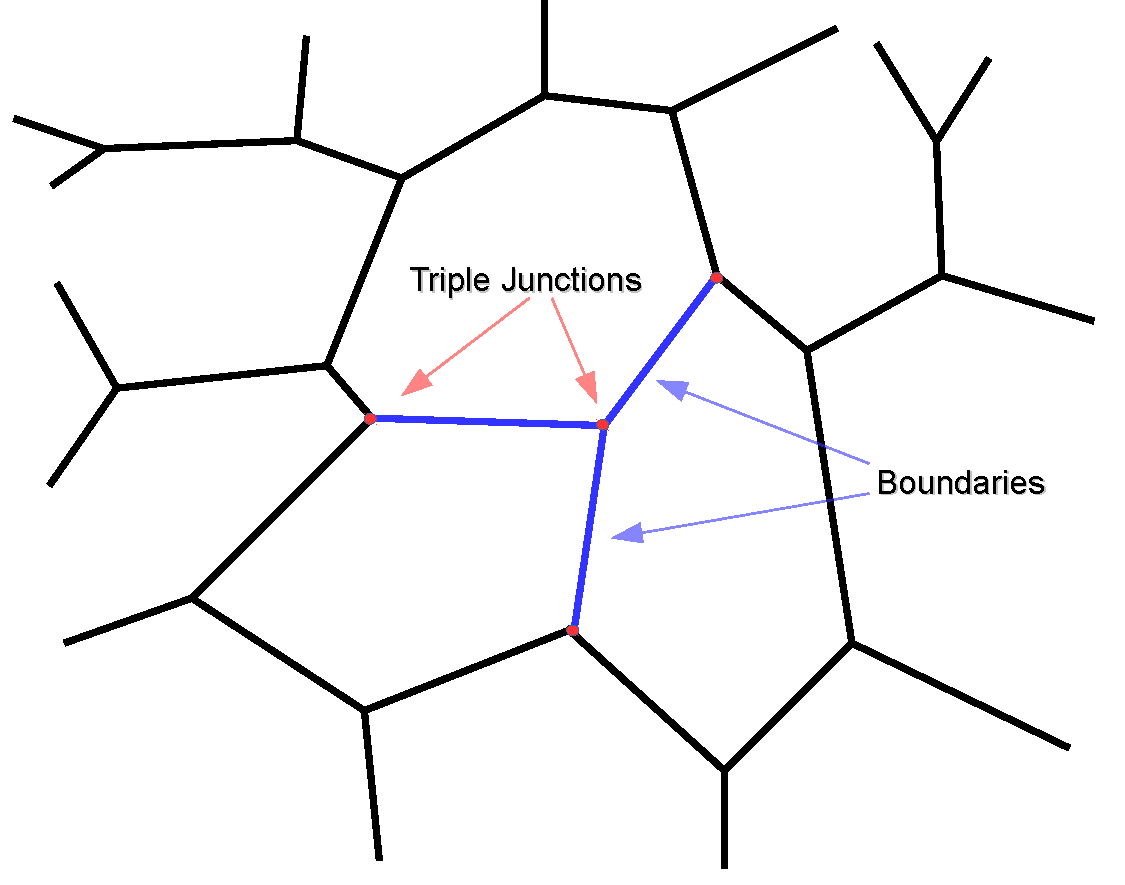
\includegraphics[scale=0.5]{scheme.pdf}
    \caption[Vertex perturbation in Stored Energy model]{Scheme of vertex modifying surrounding grains and boundaries. Arc lengths and grain areas are modified.}
    \label{fig:delta_energy}
\end{figure}

So, instead of recompute the $n$ vertex energies for each one of the $2n$ components of the gradient, we can check directly the difference of energies given by the perturbation. 
Expanding the difference of energies from \eqref{eq:partialE} and taking in account that the perturbation is local, we obtain:
\begin{align}
    E(\X+\varepsilon\,  \ei{k}) - E(\X) &=  \widehat{E}_i(\X+\varepsilon\,  \ei{k}) - \widehat{E}_i(\X) + \sum_{j \in \mathcal{N}_i}  \widehat{E}_{j}(\X+\varepsilon\,  \ei{k}) - \widehat{E}_{j}(\X)
\end{align}
The energy difference holds some common terms. For example $\widehat{E}_i(\X+\varepsilon\,  \ei{k})$ has the modified arc-lengths and areas considering that $\x_i$ moved but the stored energies and boundary energies remains constant in this time-step, thus we can use \eqref{eq:vertexenergy} and factorize $\widehat{E}_i(\X+\varepsilon\,  \ei{k}) - \widehat{E}_i(\X)$ by these constants.
\begin{equation*}
     \widehat{E}_i(\X+\varepsilon\,  \ei{k}) -  \widehat{E}_i(\X)=  \sum_{j \in \mathcal{N}_i}  \gamma_{i, j} \frac{(\Tilde{\AL}_{i,j} - \AL_{i,j})}{2} + \sum_{g \in \mathcal{G}_i} \SE_{g}\frac{(\Tilde{A}_{g} - A_{g})}{\ns(g)} ,
\end{equation*}
where $\Tilde{\AL}_{i,j}$ is the perturbed arc length for vertices $i$ and $j$ and $\Tilde{A}_{g}$ is the perturbed area of the grain $g$. The other energies terms related to neighbor vertices can be analyzed as follows. The difference $\widehat{E}_{j_1}(\X+\varepsilon\,  \ei{k}) - \widehat{E}_{j_1}(\X)$ resides in the contribution of the modified areas $\Tilde{A}_{g_1}, \Tilde{A}_{g_2}$ and the arc length $\Tilde{\AL}_{i, j_1}$. The rest of the terms remains the same in each energy term and thus are canceled, therefore:
\begin{equation}
    \widehat{E}_{j_1}(\X+\varepsilon\,  \ei{k}) - \widehat{E}_{j_1}(\X) = \gamma_{i,j_1}\frac{(\Tilde{\AL}_{i, j_1} - \AL_{i, j_1})}{2} + \SE_{g_1}\frac{(\Tilde{A}_{g_1} - A_{g_1})}{\ns(g_1)} + \SE_{g_2}\frac{(\Tilde{A}_{g_2} - A_{g_2})}{\ns(g_2)}
\end{equation}
The remaining energy differences for each neighboring vertex can be obtained analogously:
\begin{align}
    \widehat{E}_{j_2}(\X+\varepsilon\,  \ei{k}) - \widehat{E}_{j_2}(\X) &= \gamma_{i,j_2}\frac{(\Tilde{\AL}_{i, j_2} - \AL_{i, j_2})}{2} + \SE_{g_2}\frac{(\Tilde{A}_{g_2} - A_{g_2})}{\ns(g_2)} + \SE_{g_3}\frac{(\Tilde{A}_{g_3} - A_{g_3})}{\ns(g_3)}\\
    \widehat{E}_{j_3}(\X+\varepsilon\,  \ei{k}) - \widehat{E}_{j_3}(\X) &= \gamma_{i,j_3}\frac{(\Tilde{\AL}_{i, j_3} - \AL_{i, j_3})}{2} + \SE_{g_3}\frac{(\Tilde{A}_{g_3} - A_{g_3})}{\ns(g_3)} + \SE_{g_1}\frac{(\Tilde{A}_{g_1} - A_{g_1})}{\ns(g_1)}
\end{align}
Notice the common terms in all the energy differences. Adding them up we obtain that:
\begin{align}
 \widehat{E}(\X+\varepsilon\,  \ei{k}) - \widehat{E}(\X) &= \gamma_{i,j_1} \Delta \AL_{i, j_1} + \gamma_{i,j_2} \Delta \AL_{i, j_2} + \gamma_{i,j_3} \Delta \AL_{i, j_3} \nonumber\\
 &+ 3\left( \SE_{g_1}\frac{\Delta A_{g_1}}{\ns(g_1)} + \SE_{g_2}\frac{\Delta A_{g_2}}{\ns(g_2)} + \SE_{g_3}\frac{\Delta A_{g_3}}{\ns(g_3)}\right).
 \label{eq:diffenergy}
\end{align}
Therefore we just need to compute the new arc lengths and areas and their differences.

Moreover, each estimation of the gradient can be computed in parallel maintaining the local information of temporal areas and arc lengths without overwriting data.